%%%%%%%%%%%%%%%%%%%%%%%%%%%%%%%%%%%%%%%%%
% Article EcoFoG
% Version 2.1 (23/10/2017)
%
% adapté de :
% Stylish Article
% LaTeX Template
% Version 1.0 (31/1/13)
%
% This template has been downloaded from:
% http://www.LaTeXTemplates.com
%
% Original author:
% Mathias Legrand (legrand.mathias@gmail.com)
%
% License:
% CC BY-NC-SA 3.0 (http://creativecommons.org/licenses/by-nc-sa/3.0/)
%
%%%%%%%%%%%%%%%%%%%%%%%%%%%%%%%%%%%%%%%%%


%----------------------------------------------------------------------------------------
%	PACKAGES AND OTHER DOCUMENT CONFIGURATIONS
%----------------------------------------------------------------------------------------

\documentclass[fleqn,10pt]{ArtEcoFoG} % Document font size and equations flushed left

\setcounter{tocdepth}{3} % Show only three levels in the table of contents section: sections, subsections and subsubsections


% Pandoc environments
\usepackage{framed}
\usepackage{fancyvrb}
\providecommand{\tightlist}{%
  \setlength{\itemsep}{0pt}\setlength{\parskip}{0pt}}
\newcommand{\VerbBar}{|}
\newcommand{\VERB}{\Verb[commandchars=\\\{\}]}
\DefineVerbatimEnvironment{Highlighting}{Verbatim}{commandchars=\\\{\}, fontsize=\scriptsize} % Code R
\definecolor{shadecolor}{RGB}{248,248,248}
\newenvironment{Shaded}{\begin{snugshade}}{\end{snugshade}}
\newcommand{\KeywordTok}[1]{\textcolor[rgb]{0.13,0.29,0.53}{\textbf{{#1}}}}
\newcommand{\DataTypeTok}[1]{\textcolor[rgb]{0.13,0.29,0.53}{{#1}}}
\newcommand{\DecValTok}[1]{\textcolor[rgb]{0.00,0.00,0.81}{{#1}}}
\newcommand{\BaseNTok}[1]{\textcolor[rgb]{0.00,0.00,0.81}{{#1}}}
\newcommand{\FloatTok}[1]{\textcolor[rgb]{0.00,0.00,0.81}{{#1}}}
\newcommand{\ConstantTok}[1]{\textcolor[rgb]{0.00,0.00,0.00}{{#1}}}
\newcommand{\CharTok}[1]{\textcolor[rgb]{0.31,0.60,0.02}{{#1}}}
\newcommand{\SpecialCharTok}[1]{\textcolor[rgb]{0.00,0.00,0.00}{{#1}}}
\newcommand{\StringTok}[1]{\textcolor[rgb]{0.31,0.60,0.02}{{#1}}}
\newcommand{\VerbatimStringTok}[1]{\textcolor[rgb]{0.31,0.60,0.02}{{#1}}}
\newcommand{\SpecialStringTok}[1]{\textcolor[rgb]{0.31,0.60,0.02}{{#1}}}
\newcommand{\ImportTok}[1]{{#1}}
\newcommand{\CommentTok}[1]{\textcolor[rgb]{0.56,0.35,0.01}{\textit{{#1}}}}
\newcommand{\DocumentationTok}[1]{\textcolor[rgb]{0.56,0.35,0.01}{\textbf{\textit{{#1}}}}}
\newcommand{\AnnotationTok}[1]{\textcolor[rgb]{0.56,0.35,0.01}{\textbf{\textit{{#1}}}}}
\newcommand{\CommentVarTok}[1]{\textcolor[rgb]{0.56,0.35,0.01}{\textbf{\textit{{#1}}}}}
\newcommand{\OtherTok}[1]{\textcolor[rgb]{0.56,0.35,0.01}{{#1}}}
\newcommand{\FunctionTok}[1]{\textcolor[rgb]{0.00,0.00,0.00}{{#1}}}
\newcommand{\VariableTok}[1]{\textcolor[rgb]{0.00,0.00,0.00}{{#1}}}
\newcommand{\ControlFlowTok}[1]{\textcolor[rgb]{0.13,0.29,0.53}{\textbf{{#1}}}}
\newcommand{\OperatorTok}[1]{\textcolor[rgb]{0.81,0.36,0.00}{\textbf{{#1}}}}
\newcommand{\BuiltInTok}[1]{{#1}}
\newcommand{\ExtensionTok}[1]{{#1}}
\newcommand{\PreprocessorTok}[1]{\textcolor[rgb]{0.56,0.35,0.01}{\textit{{#1}}}}
\newcommand{\AttributeTok}[1]{\textcolor[rgb]{0.77,0.63,0.00}{{#1}}}
\newcommand{\RegionMarkerTok}[1]{{#1}}
\newcommand{\InformationTok}[1]{\textcolor[rgb]{0.56,0.35,0.01}{\textbf{\textit{{#1}}}}}
\newcommand{\WarningTok}[1]{\textcolor[rgb]{0.56,0.35,0.01}{\textbf{\textit{{#1}}}}}
\newcommand{\AlertTok}[1]{\textcolor[rgb]{0.94,0.16,0.16}{{#1}}}
\newcommand{\ErrorTok}[1]{\textcolor[rgb]{0.64,0.00,0.00}{\textbf{{#1}}}}
\newcommand{\NormalTok}[1]{{#1}}
\usepackage{longtable,booktabs}
\usepackage{caption}
% These lines are needed to make table captions work with longtable:
\makeatletter
\def\fnum@table{\tablename~\thetable}
\makeatother
% longtable 2 columns
% https://tex.stackexchange.com/questions/161431/how-to-solve-longtable-is-not-in-1-column-mode-error
\makeatletter
\let\oldlt\longtable
\let\endoldlt\endlongtable
\def\longtable{\@ifnextchar[\longtable@i \longtable@ii}
\def\longtable@i[#1]{\begin{figure}[t]
\onecolumn
\begin{minipage}{0.5\textwidth}\scriptsize
\oldlt[#1]
}
\def\longtable@ii{\begin{figure}[t]
\onecolumn
\begin{minipage}{0.5\textwidth}\scriptsize
\oldlt
}
\def\endlongtable{\endoldlt
\end{minipage}
\twocolumn
\end{figure}}
\makeatother

\usepackage{graphicx,grffile}
\makeatletter
\def\maxwidth{\ifdim\Gin@nat@width>\linewidth\linewidth\else\Gin@nat@width\fi}
\def\maxheight{\ifdim\Gin@nat@height>\textheight0.8\textheight\else\Gin@nat@height\fi}
\makeatother
% Scale images if necessary, so that they will not overflow the page
% margins by default, and it is still possible to overwrite the defaults
% using explicit options in \includegraphics[width, height, ...]{}
\setkeys{Gin}{width=\maxwidth,height=\maxheight,keepaspectratio}

% User-adder preamble
\usepackage{textcomp} \DeclareUnicodeCharacter{B0}{\textdegree}
\usepackage{tabu}
\renewenvironment{table}{\begin{table*}}{\end{table*}\ignorespacesafterend}
\hyphenation{bio-di-ver-si-ty sap-lings}

%----------------------------------------------------------------------------------------
%	ARTICLE INFORMATION
%----------------------------------------------------------------------------------------

\JournalInfo{Hal 00679993} % Journal information
\Archive{DOI xxxx} % Additional notes (e.g. copyright, DOI, review/research article)

\PaperTitle{30 Years of Post-disturbance Recruitment in Tropical Forest} % Article title

\Authors{
Ariane MIRABEL\textsuperscript{1*}\\ Eric MARCON\textsuperscript{1}\\ Bruno HERAULT\textsuperscript{2}
} % Authors
\affiliation{
\textsuperscript{1}UMR EcoFoG, AgroParistech, CNRS, Cirad, INRA, Université des Antilles,
Université de Guyane.\\ \hspace{1em} Campus Agronomique, 97310 Kourou, France.\\\textsuperscript{2}INPHB (Institut National Ploytechnique Félix Houphoüet Boigny)\\ \hspace{1em} Yamoussoukro, Ivory Coast
}
\affiliation{*\textbf{Corresponding author}: ariane.mirabel@ecofog.gf, http://www.ecofog.gf/spip.php?article47} % Corresponding author

\Keywords{Taxonomic and Functional Diversity, Recruitment, Resilience, Tropical Forests, Disturbance Dynamics} % Keywords - if you don't want any simply remove all the text between the curly brackets
\newcommand{\keywordname}{Keywords} % Defines the keywords heading name

%----------------------------------------------------------------------------------------
%	ABSTRACT
%----------------------------------------------------------------------------------------

\Abstract{
Résumé de l'article.
}

%----------------------------------------------------------------------------------------

\begin{document}

\selectlanguage{english}

\flushbottom % Makes all text pages the same height

\maketitle % Print the title and abstract box

\tableofcontents % Print the contents section

\thispagestyle{empty} % Removes page numbering from the first page

%----------------------------------------------------------------------------------------
%	ARTICLE CONTENTS
%----------------------------------------------------------------------------------------


\section{Introduction}\label{introduction}

Determining the response of tropical forests to disturbance is a key to
predict their fate in a global change context where disturbance are
expected to become more and more frequent. Tropical forests indeed
currently experience a wide range of disturbance, from radical land-use
changes for agriculture or mining \citep{Dezecache2017a, Dezecache2017b}
to insidious changes in communities structure and functioning following
changes in the precipitation regime or after selective logging
\citep{Baraloto2012a, Herault2016}. In that respect a vast literature
successfully modeled the response of tropical forests structure, carbon
stocks and fluxes to anthropogenic and natural disturbances
\citep{Gourlet-Fleury2000, Putz2012, Martin2015, Piponiot2016}.
Regarding diversity, however, similar attempts have been hindered by
both the huge biological diversity and the scarcity of long-term
monitoring. If the response to disturbance has been identified for
common species assemblages, it usually remained confined to few
commercial and valuable species
\citep{Sebbenn2008, Rozendaal2010, Vinson2015}. Forests communities
functioning and dynamics, though, result from the constantly evolving
interactions and feedbacks among trees and their environment and they
would only be assessed through the study of entire communities
\citep{DeAvila2016, Liang2016}. Forests response to disturbance is build
on the the population of disturbance survivors and the recruitment of
new individuals. The latter proved to mirror the composition of
pre-disturbance forest \citep{Herault2018} so the response of the whole
community will be driven by the diversity and composition of the
recruitment. Recruitment trajectories, directly determining the
community to be, are then key to elucidate the future of tropical forest
in the changing global environment.

Recruitment diversity and composition trajectories elucidate the
resilience of hyperdiverse tropical forest ecosystems and highlight the
determinants of their response after disturbance. To our opinion
taxonomic and functional trajectories would depend on the composition
and diversity of initial community, partly conditioning the pool of
recruited species. Thereafter, the commmunities composition will in turn
influence the assembly rules giverning further recruitment and result in
a self-perpetuated trajectory along time \citep{Kunstler2016}. Similar
reasoning apply to both taxonomic and functional trajectories, although
given the possible decoupling between taxonomic and functional
characteristics in a community their respective trajectories might
differ \citep{Fukami2005}. The dependency of communties trajectories
upon their initial state besides brings the question of its resilience,
meaning the convergence of communities towards pre-disturbance
conditions and the maintenance of the initial differences among
communities \citep{Diaz2005, Gardner2007, Schwartz2017}. In addition to
those intrinsinc communities parameters, the recruitment results from
the interplay of external processes either stochastic, like random
dispersal, recruitment and death \citep{Hubbell2001}, or deterministic
like niche-based competition processes \citep{Adler2007}. While
stochastic processes would build communities as random samples of
larger, regional ones, deterministic processes rely on the abiotic
environment and filter-out recruited species according to their ecology.
Specifically, species would be selected through their tolerance to
stress or competition for resources. Based on the Intermediate
Disturbance Hypothesis (IDH) these deterministic processes and the
patchy variability of environmental conditions in space and time
maintain a large ecological range in the community via the species
selected under past environmental conditions \citep{Guitet2018}. In
tropical forests deterministic processes depend on the strategy of
resource use, specifically light, and therefore result in shifts from
fast growing, resources-acquisitive but stress-intolerant species
favored in disturbance gaps, to slow-growing, stress-tolerant and
resource-conservative species dominating in mature forests
\citep{Denslow1980, Molino2001, Bongers2009}. Communities functional
diversity would then be driven either by selective pressures
filtering-out some functional strategies or by the competitive exclusion
for resources limiting the functional similarity among species
\citep{Ackerly2003, McGill2006}. It would be translated by either the
overdispersion or the restriction of leaf and stem functional traits
(leaf thickness, toughness, chlorophyll content and specific area; wood
specific gravity and bark thickness) and life-history traits (maximum
height at adult stage and class of seed mass)
\citep{Wright2004, Chave2009b, Herault2011}.

Empirical tests of those mechanisms, the validation of the IDH in
tropical rainforests, and the resilience of communities proved hard to
succeed and yielded controversial results
\citep{Hubbell1999, Molino2001, Sheil2003}. In this paper we follow the
fate of a recruited tree communities (60121 individuals) over 30 years
on a disturbance gradient, with 10 to 60\% of forest biomass removed. We
assessed the taxonomic as well as functional diversity of recruited
trees, using a large functional trait database covering the leaf, wood
and life-history spectra. We compared the observed trajectories to null
models representing random trees recruitment and randomized functional
traits. We aimed to (i) assess the role of deterministic processes
compared to stochastic recruitment after disturbance, (ii) assess the
taxonomic and functional convergence of forest communities and the
maintenance of taxonomic composition in the long term, and (iii)
determine the resilience of the ecosystem.

\section{Material and Methods}\label{material-and-methods}

\subsection{Study Site}\label{study-site}

The Paracou station is located in a lowland tropical rain forest in
French Guiana (5°18'N and 52°53'W). Climate is tropical wet with mean
annual precipitation averaging 2980 mm.y\textsuperscript{-1} (30-y
period) and a 3-months dry season (\textless{} 100
mm.months\textsuperscript{-1}) from mid-August to mid-November, and a
one-month dry season in March \citep{Wagner2011}. Elevation ranges from
5 to 50 m and mean annual temperature is 26°C. Soils are thin acrisols
over a layer of transformed saprolite with low permeability generating
lateral drainage during heavy rains. The disturbance experiment spread
over a network of twelve 6.25ha plots (Table \ref{tab:Tab1}) that
underwent three disturbance treatments in 1986-1987 \citep{Herault2018}.
Dominant families are Fabaceae, Chrysobalanaceae, Lecythidaceae and
Sapotaceae.

\begin{table}

\caption{\label{tab:Tab1}Intervention table, summary of the disturbance intensity for the 4 plot treatments in Paracou.}
\centering
\begin{tabu} to \linewidth {>{\raggedright}X>{\raggedright}X>{\raggedright}X>{\raggedright}X>{\raggedright}X}
\toprule
Treatment & Timber & Thinning & Fuelwood & \%AGB lost\\
\midrule
Control &  &  &  & 0\\
T1 & DBH $\geq$ 50 cm, commercial species, $\approx$ 10 trees/ha &  &  & $[12\%-33\%]$\\
T2 & DBH $\geq$ 50 cm, commercial species, $\approx$ 10 trees/ha & DBH $\geq$ 40 cm, non-valuable species, $\approx$ 30 trees/ha &  & $[33\%-56\%]$\\
T3 & DBH $\geq$ 50 cm, commercial species, $\approx$ 10 trees/ha & DBH $\geq$ 50 cm, non-valuable species, $\approx$ 15 trees/ha & 40 cm $\leq$ DBH $\leq$ 50 cm, non-valuable species, $\approx$ 15 trees/ha & $[35\%-56\%]$\\
\bottomrule
\end{tabu}
\end{table}

\subsection{Inventories Protocol and Dataset
Collection}\label{inventories-protocol-and-dataset-collection}

All trees above 10 cm DBH were mapped and measured annually since 1984.
During inventories, trees were first identified with a vernacular name
assigned by the field team, and afterward with a scientific name
assigned by a botanist during regular botanical campaigns. Botanical
campaigns have been carried out every 5 to 6 years from 2003 onwards.
This raised methodological issues as vernacular names usually correspond
to different botanical species, resulting in significant taxonomic
uncertainties that were propagated to composition and diversity metrics.
Vernacular names were replaced through multinomial trials
\(M_v\Big(\big[s_1, s_2, …, s_N\big],\big[\alpha_1, \alpha_2,…, \alpha_3\big]\Big)\)
based on the observed association probability
\(\big[\alpha_1, \alpha_2,…, \alpha_3\big]\) between each vernacular
name \emph{v} and the species \(\big[s_1, s_2, …, s_N\big]\) recorded in
the inventory. See appendix 1 and \citet{Aubry-Kientz2013} for the
detailed methodology. To avoid remaining identification caveats, the
simulated botanical inventories were reported at genus level.

Six functional traits, representing leaf economics (leaves thickness,
toughness, total chlorophyll content and specific leaf area, the leaf
area per unit dry mass), wood economics (wood specific gravity and bark
thickness) and life history traits (maximum specific height and seed
mass), come from the BRIDGE project \footnote{http://www.ecofog.gf/Bridge/}
where trait values were measured on nine french guianan forest plots,
including two in Paracou. Missing trait values (10\%) were filled using
multivariate imputation by chained equation (mice). As traits
variability was lower within species and within genus, we accounted for
the phylogenetic signal of the functional traits in restricting thegap
filling processes to samples pertaining to the next higher taxonomic
level (refs MICE). As seed mass information corresponds to a
classification into mass classes, no data filling process was applied so
analysis were performed only considering the 414 botanical species of
the seed mass dataset.

Functional trajectories were estimated with the Rao quadratic entropy
using community weighted means (CWM) \citep{Diaz2007, Garnier2004}. Seed
mass trajectories were reported by the proportion of each class recorded
in the inventories. All composition and diversity metrics are the
average obtained after 50 iterations of taxonomy and trait values
uncertainty propagation.

\subsection{Recruitment trajectories}\label{recruitment-trajectories}

We split the forest community in `survivors', that are the trees
surviving since disturbance, and the trees recruited after disturbance.
Two recruitment metrics were examined: on the one hand the ``punctual
recruitment'' by 2-year intervals after disturbance, on the other hand
all recruited trees since disturbance, hereafter ``accumulated
recruits''. Eventually it was to determine whether plot scale
trajectories either reflected to overall recruitment processes or were
driven by processes restricted to disturbance gaps while the recruitment
of undisturbed zones remained unchanged.

The taxonomic diversity was assessed through Richness and the Hill
number translation of Shannon and Simpson indices
\citep{Hill1973, chao2015estimating, Marcon2015b}. These three indices
belong to the set of HCDT or generalized entropy, respectively
corresponding to the 0, 1 and 2 order of diversity (\emph{q}), which
grasps the balance between richness and evenness in the community, with
common species weighting more than rare ones when \emph{q} increases.
The similarity between the recruited trees and the pre-disturbance
forest was measured with the turnover metrics detailed in
\citet{Podani2013a}. To determine whether recruitment trajectories
ensued from a random process, observed trajectories were compared to
those generated by 50 repetitions of a random null model shuffling
individuals among plots while preserving species abundance and plots'
tree density.

To draw plots trajectories we applied a moving average with a one step
(3 years) window to mitigate the heterogeneity of inventory protocols
between years.

\section{Results}\label{results}

\subsection{Recruitment Diversity}\label{recruitment-diversity}

\subsubsection{Taxonomic Diversity}\label{taxonomic-diversity}

Punctual recruits' diversity followed a consistent trajectory among
disturbance treatments with first higher richness and lower evenness
than in control plots and then equivalent richness and lower evenness
(Figure (\ref{fig:Fig1}). For recruits accumulated since disturbance,
the richness (order 0) in highly disturbed plots (T3 and some T2) was
higher than in control plots, consistently with the increase of
recruited trees after disturbance, and the evenness (order 2) was lower,
specifically for the most disturbed plots (Appendix I, fig. S1).

\begin{figure*}

{\centering 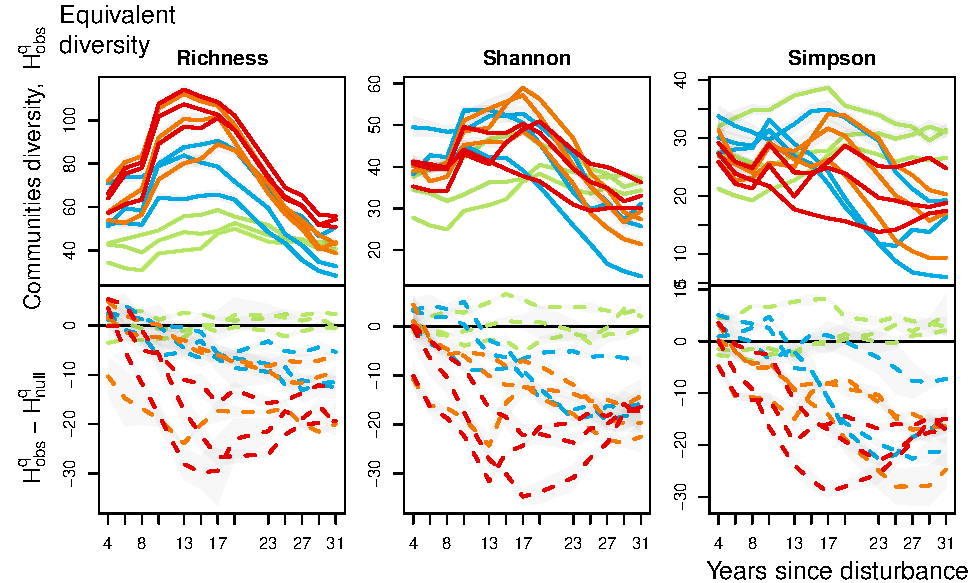
\includegraphics[width=0.8\linewidth]{RecruitmentTrajectories_files/figure-latex/Fig1-1} 

}

\caption{Trajectories of Richness, Shannon and Simpson diversity for 2-years laps punctual  recruitment (upper panels) and divergence to null model (lower panels). Lines colors refer to the perturbation regime: green for control, blue for T1, orange for T2 and red for T3 disturbance treatments. Plain lines correspond to the median observed after uncertainty propagation and are given along with the 95\% confidence interval (grey envelope).}\label{fig:Fig1}
\end{figure*}

Punctual and accumulated recruitment diversity of orders 0, 1 and 2 were
then compared to a null random recruitment model. In control plots the
richness (order 0) and evenness (order 2) of punctual recruits remained
equivalent or higher than for the null random model. For all disturbed
plots in contrast both richness and evenness were lower than these of a
random null model but displayed a significant but unachieved
humped-shaped trajectory for all plots (Figure \ref{fig:Fig1}).
Accumulated recruitment richness and evenness were higher or equivalent
to those of the null model for plots T1 and some plots T2 but lower for
plots T3 and a plot T2 (AppendixI, fig. S1).

The trajectories obtained

\subsubsection{Functional Diversity and
Composition}\label{functional-diversity-and-composition}

The functional diversity (Rao diversity) of punctual recruitment was
measured and compared to a null model of random traits shuffling. In
most distrubed plots (plots T2 and T3) the functional diversity was
deacrinsing and lower to this of control plots until 15 years after
disturbance (Figure \ref{fig:Fig3}). It then increased to values
equivalent or higher to those observed in control plots. For all
disturbed and control plots the observed functional diversity was lower
than for the null model of random traits shuffle, except for two T1
plots.

\begin{figure}

{\centering 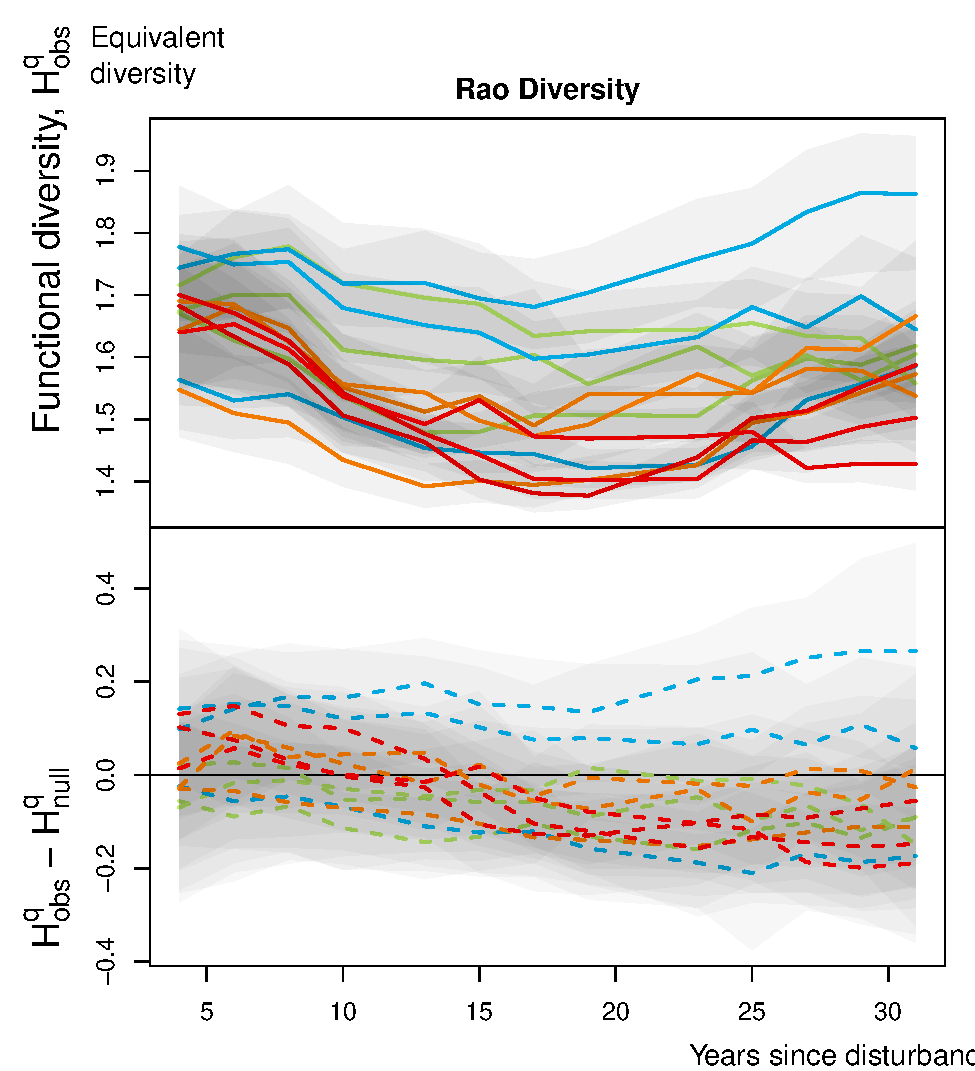
\includegraphics{RecruitmentTrajectories_files/figure-latex/Fig2-1} 

}

\caption{Functional diversity of punctual recruited trees from the considered functional traits and divergence to null model. Values reported correspond to the plot-level median and the 95\% confidence interval obtained after 50 repetition of the taxonomic uncertainty propagation and the functional database gap-filling processes and 50 run of the null model. Lines colors correspond to the logging treatment initially applied (green for control, blue for T1,orange for T2 and red for T3).}\label{fig:Fig2}
\end{figure}

Trajectories of recruited trees in the functional spaces showed the
dominance after disturbance of species displaying large exchange surface
area and light tissues (high SLA, low leaf toughnessand thickness and
low wood specific gravity) (Figure \ref{fig:Fig3}). All traits
trajectories displayed univariate CWM trajectories with leaf toughness,
wood specific gravity and bark thickness decreasing before stabilizing
at low values around 15 after disturbance, except SLA and leaf thickness
that displayed a unimodal trajectory with a maximum reach around 15
years after disturbance.

\begin{figure*}

{\centering 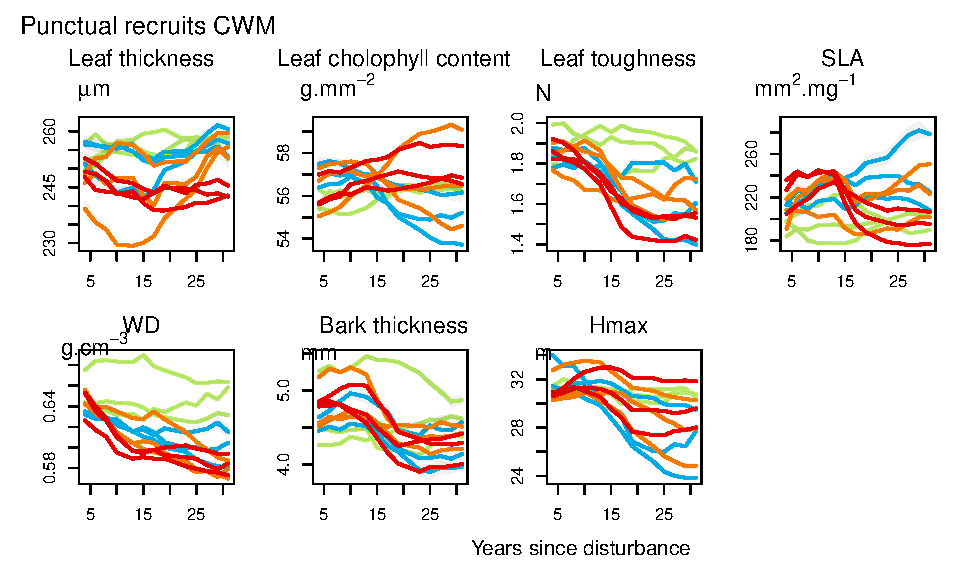
\includegraphics[width=0.8\linewidth]{RecruitmentTrajectories_files/figure-latex/Fig3-1} 

}

\caption{Community weighted means (CWM) of the four disturbance treatment for the four leaf traits, the two stem traits  and the specific Hmax. Values reported correspond to the plot-level median obtained after 50 repetition of the taxonomic uncertainty propagation and the functional database gap-filling processes. Lines colors correspond to the disturbance intensity (green for control, blue for T1,orange for T2 and red for T3).}\label{fig:Fig3}
\end{figure*}

\subsection{Recruitment Turnover}\label{recruitment-turnover}

In control plots species turnover remained highly stable for the 30
sampled years (Figure \ref{fig:Fig4}), reflecting a strong similarity
between the initial plots composition and the punctual recruits. In
disturbed plots, turnover displayed a unimodal response to disturbance,
with maximum reached around 15 years and with a value positively
correlated to the disturbance intensity (\(\rho_{spearman}=0.93\)). The
turnover trajectory returned close to zero for all plots 30 years after
disturbance.

\begin{figure}

{\centering 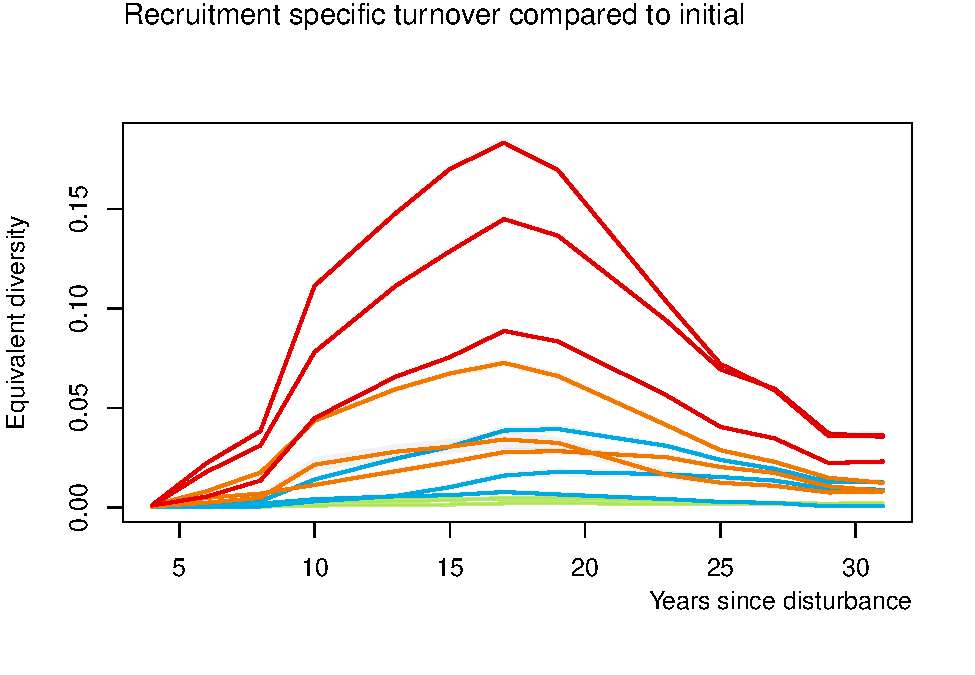
\includegraphics{RecruitmentTrajectories_files/figure-latex/Fig4-1} 

}

\caption{Trajectories over the 30 sampled years of the abundance-based turnover between recruited trees and intial communities before disturbance. Grey envelopes correspond to the 0.025 and 0.975 percentiles of the uncertainty propagation procedue and lines to the median in green for control, blue for T1,orange for T2 and red for T3).}\label{fig:Fig4}
\end{figure}

\section{Discussion}\label{discussion}

We analyzed the trajectories followed by the composition, diversity, and
functional characteristics of trees recruited after disturbance to
highlight the response of tropical forests and determine their
resilience and help future conservation strategies. The 30 years-long
monitoring analysed allowed to identify the different steps of forests
recovery and the corresponding assembly rules. We identified two
distinct phases, the first corresponding to the recruitment of
pre-disturbance saplings that reflected the diversity and composition of
the stand in place, and the second driven by ``true recruits''
germinated from the seed bank after disturbance. The second phase
involved environmental selection and progressive competition among
species according to the disturbance intensity, which build recruited
communities divergent from the initial stand persisting in the long
term.

\subsection{On the underlyings of the hump-shaped
trajectories}\label{on-the-underlyings-of-the-hump-shaped-trajectories}

The trajectories of punctual recruitment richness, of some key
functional traits (SLA and bark thickness) and of species turn-over
exhibited hump-shaped, unimodal trajectories.

The recruitment for 10-15 first years after disturbance did not
substantially differ from this of control plots. Recruitment
trajectories were driven by the growth of pre-disturbance saplings
benefiting from the environmental changes and alleviated competition
following disturbance \citep{Herault2010}. The functional diversity of
the recruitment remained stable after low disturbance intensity,
equating these of control plots and matching stochastic recruitment
processes. After intense disturbance, this phase brought sharp increases
in the SLA, wood density and leaf thickness trajectories. This
tendencies revealed prominent recruitment, above an intensity threshold,
of short-lived, fast growing \emph{hard pionneers} species with
competitive and efficient light acquisition (Figure \ref{fig:Fig4})
\citep{Wright2004, Chave2009b, Herault2011, Reich2014}.

Following this first phase, the recruitment progressively incorporated
true recruits, \emph{i.e.} trees germinated from the seed bank,
resulting in a decrease of recruited trees evenness and functional
diversity. A restriction in the pool of species was then recruited,
following an interplay between deterministic processes excluding less
competitive and stress-tolerant species, and stochastic recruitment as
in mature forests that progressively emerged again. The balance betwwen
both processes was determined by the intensity of the initial
disturbance. After low disturbance intensity (T1 plots), the taxonomic
composition of the recruitment resembled the pre-disturbance communities
but pool of recruited species was restricted by selective pressures on
the strategy of resource use. Favored species were more pioneers and
light demanders, with strategies of efficient resource acquisition (high
SLA and leaf chlorophyll content) and inexpensive, short-lived tissues
(low leaf thickness and thoughness, small Hmax and low wood density and
bark thickness). Correspondingly the functional diversity increased,
equating or exceeding this of control plots, which revealed an
overdispersion of the functional traits that was probably driven by the
limitation of functional similarity among species. Despite some
competitive exclusion then, recruited species still browsed a large
functional range with no high dominance of hard pionners
\citep{Hubbell1999, Sheil2003, Bongers2009}. This might due to
recruitment and dispersal limitation due to the short dispersal distance
observed for tropical trees, specifically in Paracou with the genetic
clumping of some pioneers \citep{Leclerc2015, Scotti2015a}. After
intense disturbance however, the first species recruited were hard
pioneers, which taxonomic composition highly differed from the initial
community and that generated a sharp increase for the SLA and bark
thickness weighted values. This was observed for 15 years after
disturbance, which corresponds to the life expectancy of hard pionners,
before the functional diversity increased again, acquisitive functional
still dominating, and the recruited trees progressively resembled the
initial composition and diversity. Communities trajectories then
involved the interplay between stochastic recruitment and deterministic
processes and advocated the role of disturbance to maintain forests
diversity, in line with the Intermediate Disturbance Hypothesis
\citep{Molino2001, Sheil2003}.

\subsection{On the resilience of the recruitment
process}\label{on-the-resilience-of-the-recruitment-process}

Both recruitment richness and functional diversity had recovered thirty
years after all disturbance intensity, reaching equivalent levels as
those of undisturbed forests. At that time though the recruitment remain
more important in disturbed plots and did not match the richness and
evenness of stochastic recruitment. However the divergence from
stochasticity progressively shrinked, arguing for a consistent but
long-term recovery of the recruitment process. These processes
eventually made the recruitment converging towards the initial state,
with the recruited species durably mirroring the pre-disturbance
community. More than commonly thought, the taxonomic trajectories
therefore depended on the pre-disturbance ecosystem characteristics and
leads to maintain the initial differences among communities
\citep{Anderson2007, Herault2018}. In contrast the trajectories of
traits and functional diversity were essentially similar among
treatments, arguing for the confluence of communities in the functional
space despite their divergence in taxonomic composition
\citep{Fukami2005}.

The taxonomic and functional characteristics of tropical forests were
both resilient, even if the settlment of long lived pioneers after
intense disturbance make a long term process of their recovery and still
impact communities functioning and diversity 30 years after disturbance.
This confirms previous results from the Paracou experiment, conducted 10
years \citep{Molino2001} and 20 years \citep{Baraloto2012a} after
disturbance, which suggested the resilience of taxonomic and functional
composition.

The time length of the recovery processes entails great caution
regarding the forest conservation and exploitation guidelines which
should allow a complete recovery of pre-disturbance conditions. To that
was added the involvement of the seed bank in the recovery processes
which own resilience remains unknown. Any storage effect, altering the
pool of recruitable species, would modify the resilience of the
community itself and impact the response to further disturbance events
\citep{Norden2009}. In such case, the competitive exclusion among
dormant life-stage (seeds or even seedlings) would be harsher and likely
bring more radical changes in the recruitment composition and functional
profile of the community.

\section{Conclusion}\label{conclusion}

The 30 years monitoring of the Paracou plots highlighted the tropical
forests' response to disturbance composed of two recruitment phase
modulated by the disturbance intensity. In the short-term forests
response was driven by the enhanced growth of grown saplings benefiting
from the alleviated competition and the environmental changes. Above an
intensity threshold the recruitment was besides dominated by
hard-pioneers radically changing the recruitment composition, diversity
and, likely, functioning. In the long-term response was driven by
recruits from the seed bank which underwent dselection towards light
demanding species and similarity limitation enhancing the functional
diversity. These deterministic processes followed a gradual balance with
the stochastic recruitment of mature forests which eventually restored
communities diversity and composition, maintaining their initial
differences. Although forests proved resilient to intense disturbance
this appeared to be a long-term processes likely only valid for single
disturbance events.

\begin{center}\rule{0.5\linewidth}{\linethickness}\end{center}

%----------------------------------------------------------------------------------------
%	REFERENCE LIST
%----------------------------------------------------------------------------------------

\bibliographystyle{mee}
\bibliography{references.bib}

%----------------------------------------------------------------------------------------

\end{document}
